\section{Implementation}
\SectionPage

\begin{frame}
  \frametitle{Project goals}
  \begin{itemize}
    \item Easy to extend (with modules)
      \begin{itemize}
        \item Low bar to create a module
        \item Easy to reason about how modules work together
      \end{itemize}
    \item Simple installation, for multiple OSes
    \item Modular core
    \item Good module developer experience
      \begin{itemize}
        \item Language agnostic module architecture
        \item Good debugging tools
        \item Good module library
      \end{itemize}
  \end{itemize}
\end{frame}

\begin{frame}
  \frametitle{Core}
  \begin{itemize}
    \item The core needs to
      \begin{itemize}
        \item Handle the UI and state
        \item Handle changes asynchronously
      \end{itemize}
    \item Modular; core features should be easy to swap/modify
  \end{itemize}
\end{frame}

\begin{frame}
  \frametitle{Module}
  \begin{itemize}
    \item A module needs to:
      \begin{itemize}
        \item Initialize the core state
        \item Update the core based on events
        \item Invoke other modules
      \end{itemize}
    \item A module should be \textit{stateless}
  \end{itemize}
\end{frame}

\begin{frame}
  \frametitle{Architecture}
  \begin{figure}[H]
    \centering
    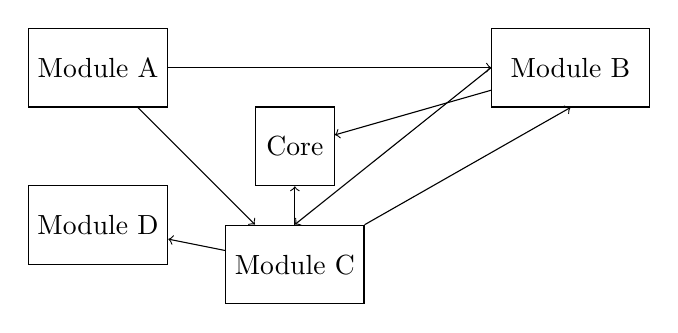
\begin{tikzpicture}
    \node (tabs) [rectangle, draw, minimum height=1cm, minimum width=1cm] at (0, 1) {Module A};
    \node (editor) [rectangle, draw, minimum height=1cm, minimum width=2cm] at (6, 1) {Module B};
    \node (fsa) [rectangle, draw, minimum height=1cm, minimum width=1cm] at (2.5, -1.5) {Module C};
    \node (cache) [rectangle, draw, minimum height=1cm, minimum width=1cm] at (0, -1) {Module D};
    \node (core) [rectangle, draw, minimum height=1cm, minimum width=1cm] at (2.5, 0) {Core};

    \draw[->] (tabs) to node[midway, above] {} (editor);
    \draw[->] (tabs) to node[midway, above] {} (fsa);
    \draw[->] (editor.west) to node[midway, above] {} (fsa.north);
    \draw[->] (editor) to node[midway, above] {} (core);
    \draw[->] (fsa) to node[midway, below] {} (editor.south);
    \draw[->] (fsa) to node[midway, above] {} (cache);
    \draw[->] (fsa) to node[midway, above] {} (core);
\end{tikzpicture}
    \caption{
      Diagram of the application architecture, note how this is similar to an
      microservice architecture
    }
  \end{figure}
\end{frame}

\begin{frame}
  \frametitle{Techstack}
  \begin{itemize}
    \item Rust with Tauri
    \item JavaScript for UI
    \item Supports all languages targeting JavaScript and Rust
  \end{itemize}
\end{frame}

\begin{frame}
  \frametitle{Core implementation}
  \begin{itemize}
    \item Modules send core modifications
    \item Instruction set on how the core is modified
    \item Modifies the state and the UI
    \item Is like a semigroup
    \item $(Instr_0 \odot Instr_1) \odot Instr_3 = Instr_0 \odot (Instr_1 \odot Instr_3)$
  \end{itemize}
\end{frame}

\begin{frame}
  \frametitle{Different hats}
  \begin{itemize}
    \item Module developer
    \item Core developer
    \item Platform developer
      \begin{itemize}
        \item User interactions through HTML-API
        \item Event-handler
        \item Events are in the same context
      \end{itemize}
  \end{itemize}
\end{frame}

\begin{frame}
  \frametitle{Module example in TypeScript}
  \begin{center}
    \lstinputlisting
    [ language=TypeScript
    ]{./code/module.ts}
  \end{center}
\end{frame}

\begin{frame}
  \frametitle{Counter module example: init}
  \begin{center}
    \lstinputlisting
    [ language=TypeScript
    ]{./code/module-counter-init.ts}
  \end{center}
\end{frame}

\begin{frame}
  \frametitle{Counter module example: handler}
  \begin{center}
    \lstinputlisting
    [ language=TypeScript
    ]{./code/module-counter-handler.ts}
  \end{center}
\end{frame}